\documentclass[aspectratio=169,
				xcolor=table]{beamer}

% Load general definitions
\usepackage[utf8]{inputenc}
%\usepackage[T1]{fontenc}
\usepackage[brazil]{babel}
\usepackage{amsmath}
\usepackage{amsfonts}
\usepackage{amssymb}
\usepackage{graphicx}
\usepackage{verbatim}
\usepackage{cancel}
\usepackage{askmaps}
\usepackage{tabularx}
\usepackage[table]{xcolor}
%\usepackage{tikz}
\usepackage{multirow}
\usepackage{mathtools}
\usepackage{color, colortbl}
\usepackage{etoolbox}
\usepackage{pbox}
\usepackage{changepage}
\usepackage{xpatch}
\usepackage{array}
\usepackage{marvosym}
\usepackage{tabu}
\usepackage{multicol}
\usepackage{listings}
\usepackage{underscore}
\usepackage{filecontents}
\usepackage[]{algorithm2e}
\usepackage{ragged2e}

\newcolumntype{P}[1]{>{\centering\arraybackslash}m{#1}}
\definecolor{Gray}{gray}{0.75}
\definecolor{Gray2}{gray}{0.85}

\definecolor{lightBlue}{HTML}{DAE8FC}
\definecolor{Blue}{RGB}{51, 51, 204}

%\useinnertheme[lily]{rounded}
\usetheme{UniEvangelica}
%\usetheme{Copenhagen}
%\usetheme{Berlin}
%\usecolortheme{dolphin}
\tolerance=1
\emergencystretch=\maxdimen
\hyphenpenalty=10000
\hbadness=10000

\setbeamertemplate{navigation symbols}{}%remove navigation symbols


\let\olditem=\item% 
\renewcommand{\item}{\olditem \justifying}%
\def\center{\trivlist \centering\item\relax}
\def\endcenter{\endtrivlist}

\setbeamertemplate{itemize/enumerate body begin}{\large}
\setbeamertemplate{itemize/enumerate subbody begin}{\large}

\setbeamertemplate{itemize item}{\raisebox{0.1ex}{$\blacktriangleright$}\hskip0.1em}
\setbeamertemplate{itemize subitem}{\raisebox{0.1ex}{$\blacktriangleright$}\hskip0.1em}

\newcommand{\greenarrow}{\textcolor{green}{\rotatebox[origin=c]{180}{\MVArrowDown}}}

\newcommand{\redarrow}{\textcolor{red}{\MVArrowDown}}

%\newcommand{\ftable}{
%	\begin{table}
%		\large
%		\centering
%		\rowcolors{1}{\ifnumless{\rownum}{2}{Blue}{lightBlue}}{}
%}

\newenvironment{eftable}{
	\begin{table}
		\large
		\centering
		\rowcolors{1}{}{Blue}
		\rowcolors{1}{\ifnumless{\rownum}{2}{Blue}{lightBlue}}{}
	}
	{
	\end{table}
}


%\setbeamertemplate{frametitle}
%{
%	%\vspace*{-2em}	
%	\insertframetitle
%
%	 %\textcolor{white}{\LARGE \insertframetitle}
%
%}

% Specific definitions
\institute[]{\uppercase{Engenharia de Software}}
\title[]{Arquitetura e Organização de Computadores}
\subtitle[]{\uppercase{Sistemas de Numeração}}
\author[]{Prof. Alexandre Tannus}
\date{}

%\AtBeginSection{\frame{\sectionpage}}

\begin{document}

	\begin{frame}
		\titlepage
	\end{frame}

	\begin{frame}
		\tableofcontents		
	\end{frame}	

	\begin{frame}{Objetivos}
		\begin{itemize}
			\item Apresentar os conceitos de sistemas de numeração
			\vspace{1em}
			\item Conhecer os sistemas decimal, binário, octal e hexadecimal
			\vspace{1em}
			\item Calcular as conversões entre os sistemas estudados
		\end{itemize}
	\end{frame}

	\section{Introdução}
		\begin{frame}
			\frametitle{Introdução}
			\begin{itemize}
				\item \textit{Design} digital é a manipulação ordenada de sinais digitais por componentes de \textit{hardware}
	%			\pause			
				\item \alert{Unidade fundamental}: dígito binário – \textbf{bit}
			\end{itemize}			
		\end{frame}

	\section{Sistemas de Numeração}	
		\begin{frame}
			\frametitle{Notações}
			\begin{itemize}
				\item Representação de números em diferentes bases
				\begin{itemize}
					\item $(numero)_{base}$
				\end{itemize}
				\vspace{1em}
				\item Exemplos
				\begin{itemize}
					\item $(94)_{10}$
					\item $(75)_{8}$
					\item $(C8)_{16}$
					\item $\alert{(100111)_{2}}$
	
				\end{itemize}
				
			\end{itemize}
		\end{frame}
%	\subsection{Sistema Decimal}	
		\begin{frame}
			\frametitle{Sistema Decimal}
			\begin{itemize}
				\item Símbolos: 0, 1, 2, 3, 4, 5, 6, 7, 8, 9
	
			\end{itemize}
		\end{frame}
		
		\begin{frame}
			\frametitle{Sistema Decimal}
			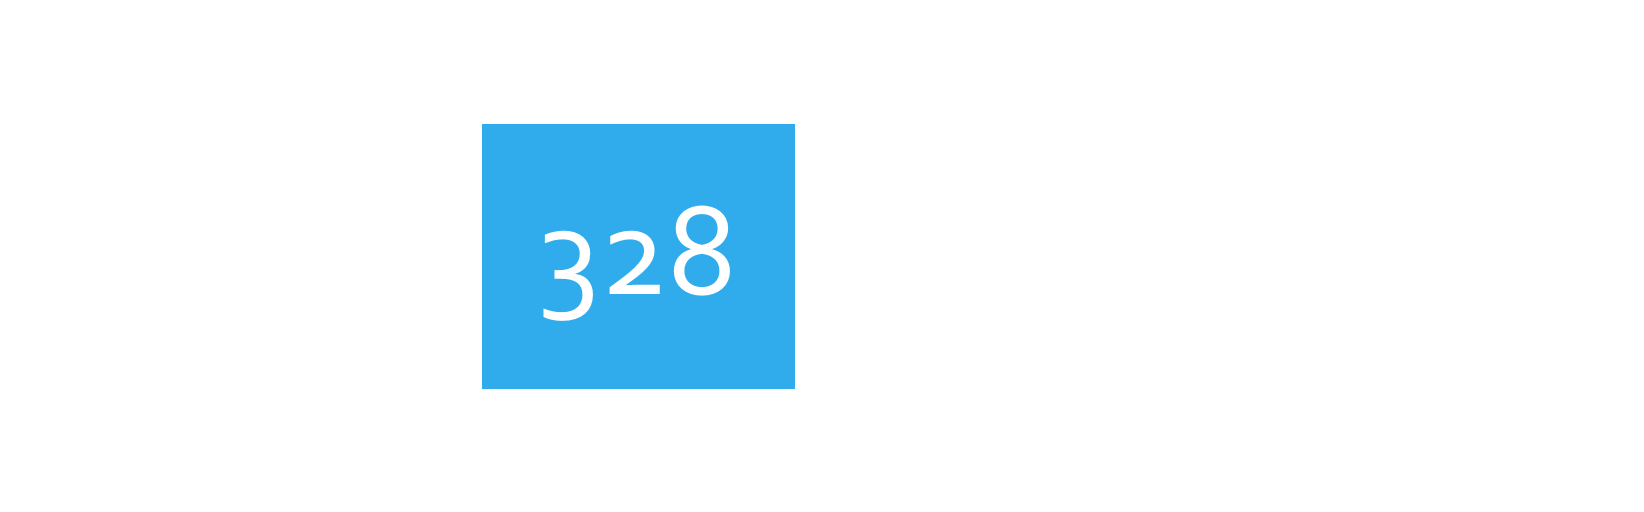
\includegraphics[width=\textwidth, keepaspectratio]{../figs/cap02/decimal01.png} 		
		\end{frame}
	
		\begin{frame}
			\frametitle{Sistema Decimal}
			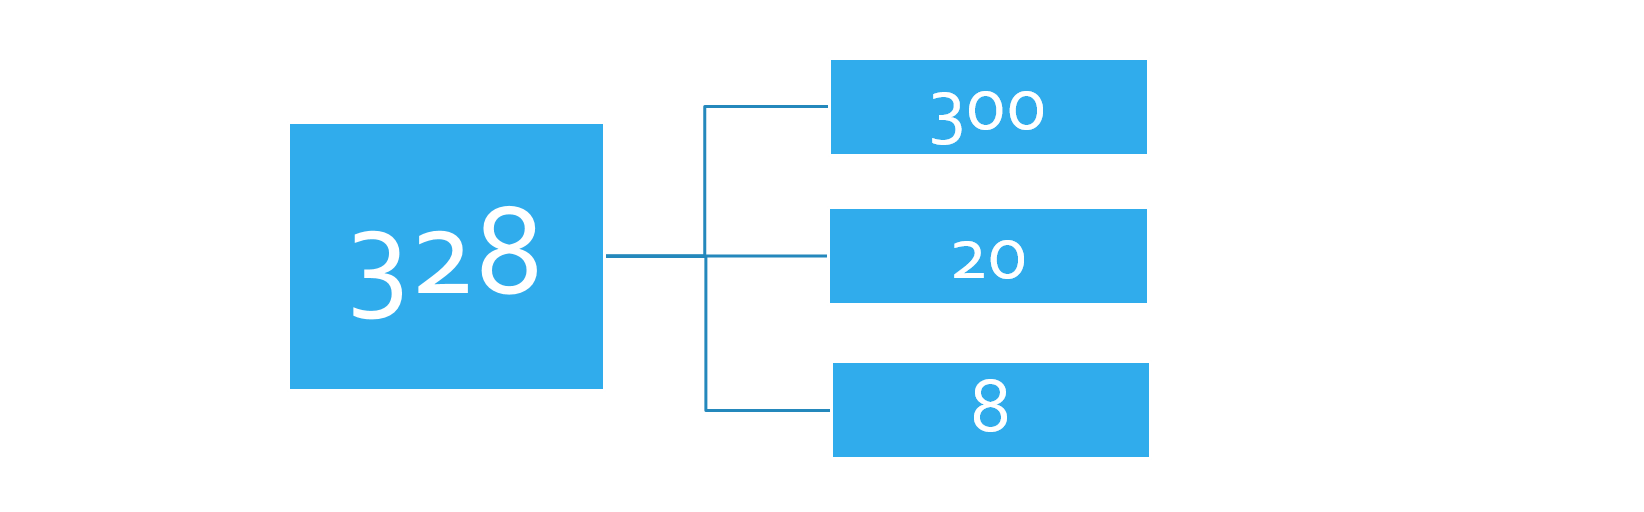
\includegraphics[width=\textwidth, keepaspectratio]{../figs/cap02/decimal02.png}  		
		\end{frame}
	
		\begin{frame}
			\frametitle{Sistema Decimal}
			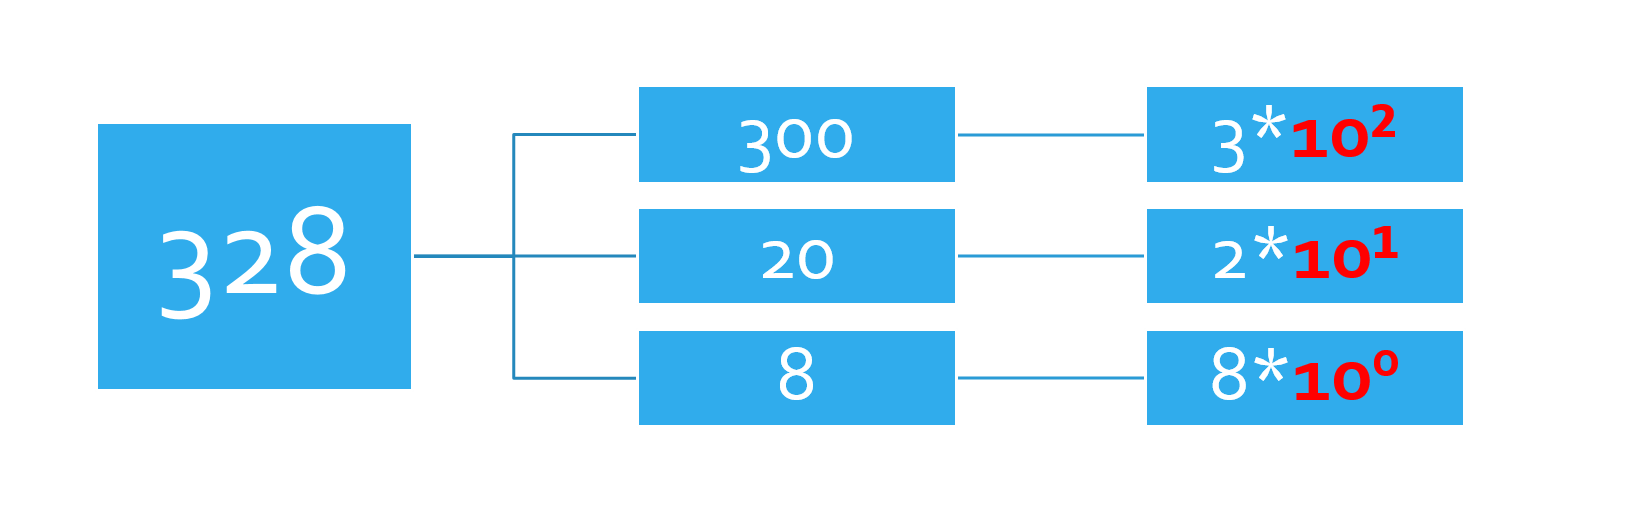
\includegraphics[width=\textwidth]{../figs/cap02/decimal03.png} 		
		\end{frame}
		
%	\subsection{Sistema Binário}	
		\begin{frame}
			\frametitle{Sistema Binário}
			\begin{itemize}
				\item Símbolos: 0, 1			
				\vspace{0.5cm}
	%			\pause
				\item Conversão Binário $\to$ Decimal
				\begin{itemize}
					\item O valor de cada símbolo é multiplicado pelo expoente relativo à sua posição (como fizemos no sistema decimal)
				\end{itemize}			
				\vspace{0.5cm}
	%			\pause
				\item Conversão Decimal $\to$ Binário
				\begin{itemize}
					\item Divisões sucessivas
					\item Soma
				\end{itemize}
			\end{itemize}
		\end{frame}
	
		\begin{frame}
			\frametitle{Sistema Binário}
			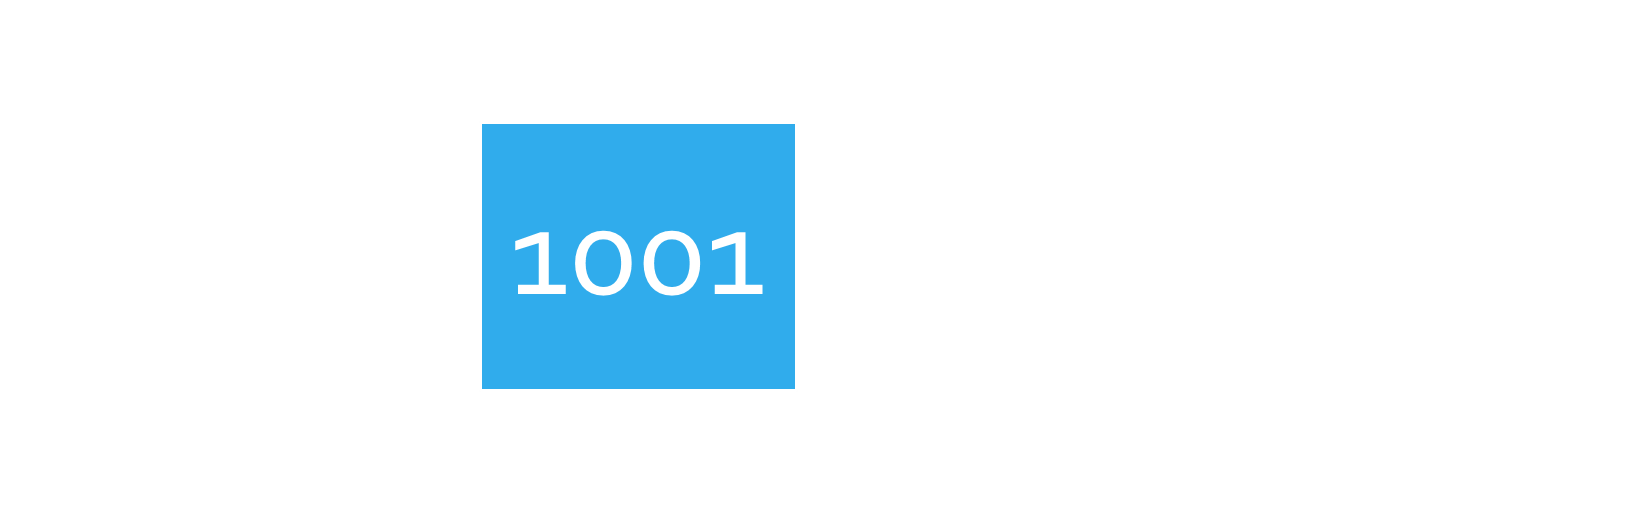
\includegraphics[width=\textwidth, keepaspectratio]{../figs/cap02/binario01.png} 		
		\end{frame}
	
		\begin{frame}
			\frametitle{Sistema Binário}
			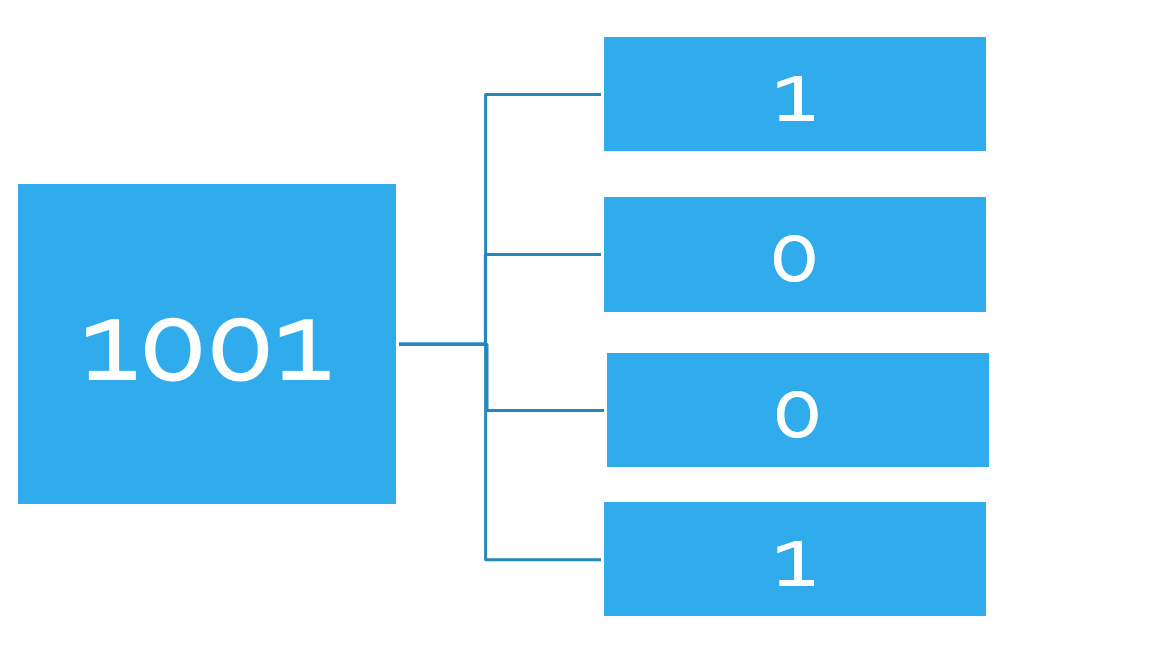
\includegraphics[width=0.8\textwidth, keepaspectratio]{../figs/cap02/binario02.png} 		
		\end{frame}
	
		\begin{frame}
			\frametitle{Sistema Binário}
			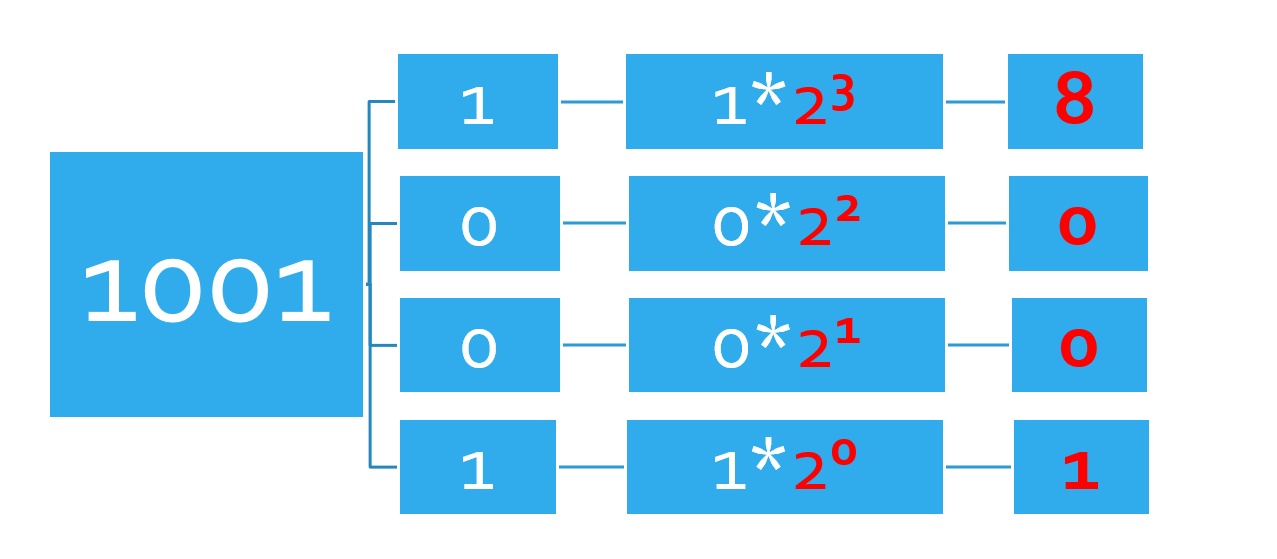
\includegraphics[width=\textwidth, keepaspectratio]{../figs/cap02/binario03.png} 		
		\end{frame}	
		
		
%	\subsection{Sistema Hexadecimal}	
		\begin{frame}
			\frametitle{Sistema Hexadecimal}
			\begin{itemize}
				\item Símbolos: 0, 1, 2, 3, 4, 5, 6, 7, 8, 9, A, B, C, D, E, F
				\vspace{1em}
				
				\item Conversão Hexadecimal $\to$ Binário
				\begin{itemize}
					\item Cada \alert{símbolo hexadecimal} equivale a \alert{quatro dígitos binários}\\
				\end{itemize}
				\vspace{1em}
				
				\item Conversão Hexadecimal $\to$ Decimal
				\begin{itemize}
					\item O valor de cada símbolo é multiplicado pelo expoente relativo à sua posição (como fizemos no sistema decimal)
				\end{itemize}
			\end{itemize}
		\end{frame}
		
		\begin{frame}
			\frametitle{Tabela de Conversão}
			
			\begin{columns}
				\begin{column}{0.45\paperwidth}
					\begin{eftable}
						\begin{tabular}{l|l|l}
							\textcolor{white}{Decimal} & 
							\textcolor{white}{Binário} & 
							\textcolor{white}{Hexadecimal} \\
							0 & 0000 0000 & 00 \\
							1 & 0000 0001 & 01 \\
							2 & 0000 0010 & 02 \\
							3 & 0000 0011 & 03 \\
							4 & 0000 0100 & 04 \\
							5 & 0000 0101 & 05 \\
							6 & 0000 0110 & 06 \\
							7 & 0000 0111 & 07 \\
							8 & 0000 1000 & 08 \\
							9 & 0000 1001 & 09 \\
						
						\end{tabular}
					\end{eftable}
				\end{column}
				\begin{column}{0.45\paperwidth}
					\begin{eftable}
						\begin{tabular}{l|l|l}
							\textcolor{white}{Decimal} & 
							\textcolor{white}{Binário} & 
							\textcolor{white}{Hexadecimal} \\
							10 & 0000 1010 & 0A \\
							11 & 0000 1011 & 0B \\
							12 & 0000 1100 & 0C \\
							13 & 0000 1101 & 0D \\
							14 & 0000 1110 & 0E \\
							15 & 0000 1111 & 0F \\
							16 & 0001 0000 & 10 \\
							17 & 0001 0001 & 11 \\
							18 & 0001 0010 & 12 \\
							19 & 0001 0011 & 13 \\
							
						
						\end{tabular}
					\end{eftable}
				\end{column}
			\end{columns}
		\end{frame}	
			
%	\subsection{Sistema Octal}	
		\begin{frame}
			\frametitle{Sistema Octal}		
			\begin{itemize}
				\item Símbolos: 0, 1, 2, 3, 4, 5, 6, 7
				\vspace{1cm}
	%			\pause
				\item Conversão Octal $\to$ Binário
				\begin{itemize}
					\item Cada \alert{símbolo octal} equivale a \alert{três dígitos binários}\\
				\end{itemize}
				\vspace{1cm}
			
	%			\pause
				\item Conversão Octal $\to$ Decimal
				\begin{itemize}
					\item O valor de cada símbolo é multiplicado pelo expoente relativo à sua posição (como fizemos no sistema decimal)
				\end{itemize}
			\end{itemize}
		\end{frame}
	
		
%	\subsection{Regras de conversão}		
		\begin{frame}
			\frametitle{Regras gerais de conversão}
			\begin{itemize}
				\item Decimal $\to$ Binário / Hexadecimal / Octal
				\begin{itemize}
					\item Divisões sucessivas pela base\\
				\end{itemize}
				\vspace{0.2cm}
	%			\pause
				\item Binário / Hexadecimal / Octal $\to$ Decimal
				\begin{itemize}
					\item Multiplicação do valor do símbolo pelo expoente relativo à sua posição\\
				\end{itemize}
				\vspace{0.2cm}
	%			\pause
				\item Hexadecimal $\leftrightarrow$ Binário 
				\begin{itemize}
					\item Símbolo hexadecimal equivale a quatros bits\\
				\end{itemize}
				\vspace{0.2cm}
	%			\pause
				\item Octal $\leftrightarrow$ Binário 
				\begin{itemize}
					\item Símbolo octal equivale a três bits\\
				\end{itemize}
				\vspace{0.2cm}
	%			\pause
				\item Octal $\leftrightarrow$ Hexadecimal
				\begin{itemize}
					\item \alert{\textbf{NÃO FAZER}}
				\end{itemize}
				\vspace{0.2cm}
			\end{itemize}
		\end{frame}
		
	\begin{frame}{Bibliografia}
		\nocite{Stallings2010}
    	\bibliographystyle{plain}
    	\bibliography{../refs}   	
	
	\end{frame}		

	\begin{frame}{}
	\end{frame}

\end{document}
